\documentclass[conference]{IEEEtran}
%\renewcommand{\thesubsection}{\thesection.\alph{subsection}}

%\addtolength{\oddsidemargin}{-.875in}
%\addtolength{\evensidemargin}{-.875in}
%\addtolength{\textwidth}{1.75in}
%\addtolength{\topmargin}{-.875in}
%\addtolength{\textheight}{1.75in}
	
\usepackage{bm}
\usepackage{amsmath}
\usepackage{amssymb}
\usepackage{tikz}
\usetikzlibrary{automata,positioning}
\usepackage{url}
\usepackage{float}
\usepackage{setspace}
\usepackage{filecontents,lipsum}
\usepackage[noadjust]{cite}

\begin{document}
%\raggedright
%\doublespacing

\title{Week 3 Journal}
\author{Rodger Byrd}
\maketitle


\section{Topic Map}
For my area I'm looking at Anti-Patterns in code, these are also known as code smells. I've also seen them referred to as Atoms of Confusion and nano patterrns. My topic map is included below in figure \ref{fig:TM}. 
\begin{figure*}
  \centerline{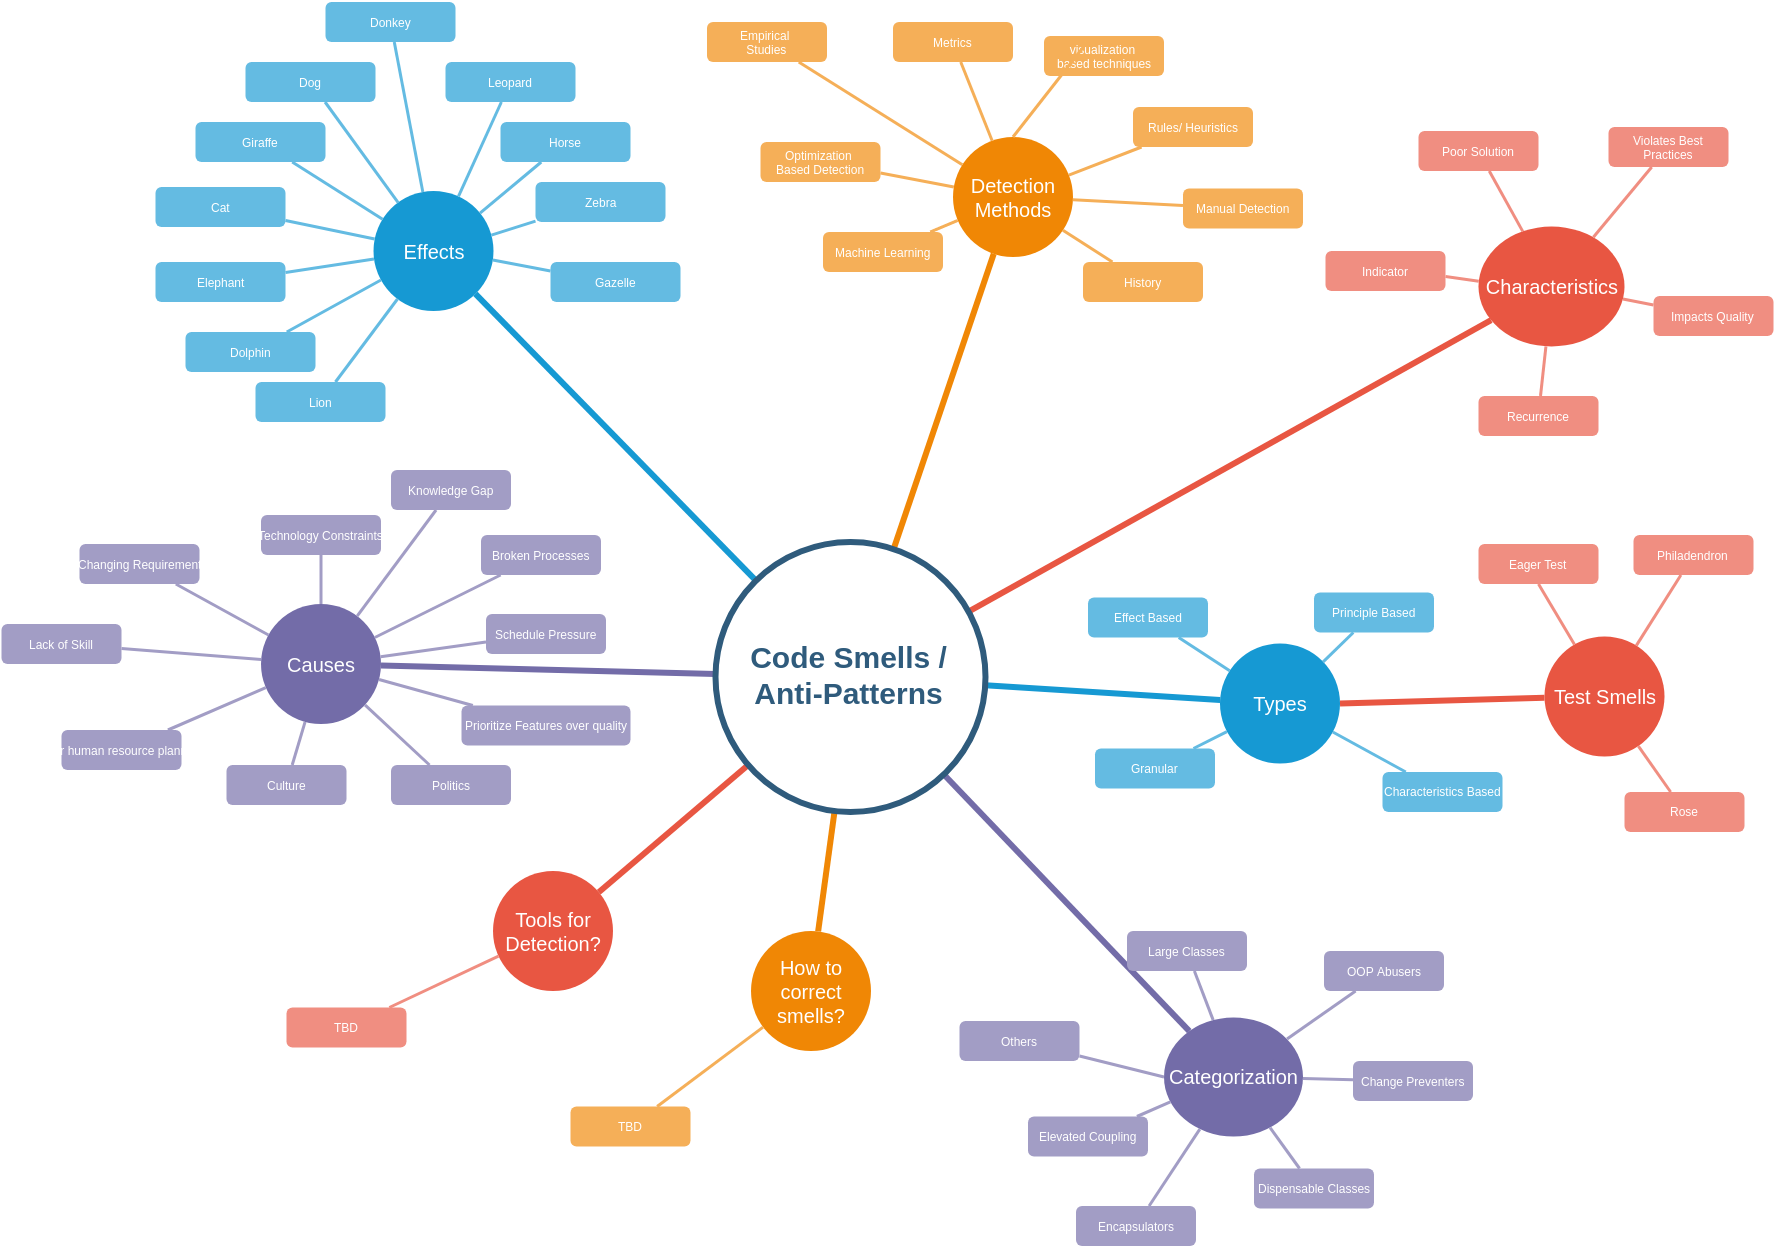
\includegraphics[width=\textwidth]{codesmells.png}}
  \caption{TopicMap}
  \label{fig:TM}
\end{figure*} 

\section{Notes on Survey Papers, }
For my first detailed read I chose a paper called  \textit{A survey on software smells} \cite{sharma_survey_2018}.The following are my raw notes for this paper.

Kent Beck coined the term code smell, I should look at this paper.
Contains some ideas for topic map in abstract.
Figure 1 in paper has a pretty detailed topic map.
Interesting for comparison.
Table 4 code smells.
Interesting section on whether anti-patterns and smells synonyms, doesn't seem to be consensus. Some papers yes, some no.
Smell indicator of problem, anti pattern definitive problem.
Current detection methods cause too many false positives?


For my next detailed read I chose a paper called  \textit{A systematic literature review: Refactoring for disclosing code smells in object oriented software} \cite{singh_systematic_2018}. The following are my raw notes for this paper.


The files for this latex document are in the github repository located at \path{https://github.com/rodger79/CS6000}

Papers that were scanned and trashed are referenced in the bibliography below. 
\nocite{*}

\bibliographystyle{IEEEtran}
\bibliography{references}


\end{document}